\section{Simulazioni MIL}
Nella seguente sezione verranno commentati i risultati delle simulazioni utilizzando i modelli di controllo mostrati nel capitolo (\ref{cap:controllore}), utilizzando i segnali analoghi alle simulazioni SIL. La modellazione dei sensori e dello stimatore utilizzato è lo stesso mostrato nella tesi \cite{DesTestCarm}. 

\subsection{PID}
La seguente simulazione utilizza il controllore PID eseguendo la traiettoria generata dalla sequenza di waypoint SNAKE.
\begin{figure}
	\centering
	\begin{subfigure}{0.45\textwidth}
		\centering
		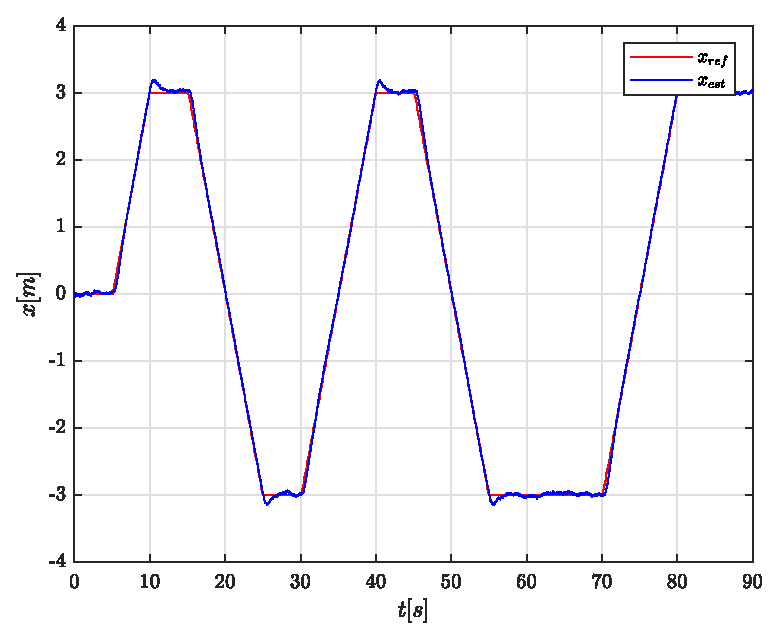
\includegraphics[width=1\textwidth]{Simulazioni/Figure/PID/SNAKE_MIL/PositionControlXPos}
		\caption{Controllo posizione lungo x}
		\label{fig:SNAKEerrposxPID_MIL}
	\end{subfigure}
	\hfill
	\begin{subfigure}{0.45\textwidth}
		\centering
		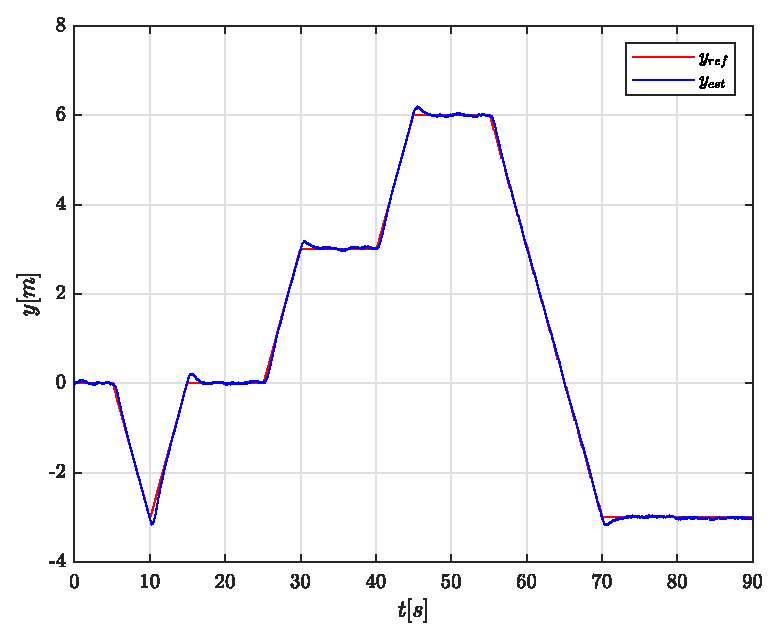
\includegraphics[width=1\textwidth]{Simulazioni/Figure/PID/SNAKE_MIL/PositionControlYPos}
		\caption{Controllo posizione lungo y}
		\label{fig:SNAKEerrposyPID_MIL}
	\end{subfigure}
	\caption{Risposta nella simulazione MIL in posizione con controllore PID al comando SNAKE}
\end{figure}

\begin{figure}
	\centering
	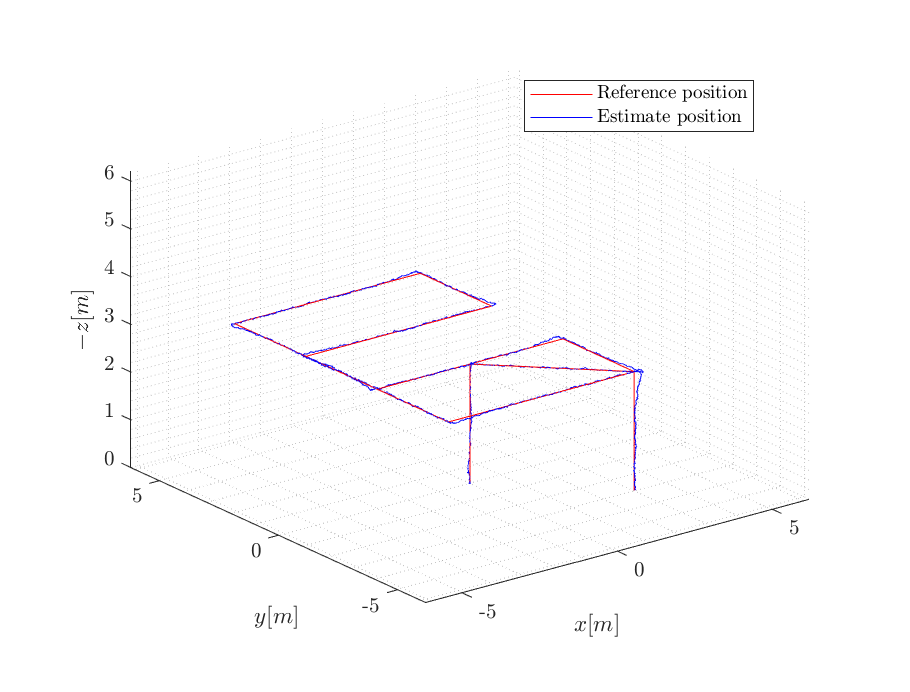
\includegraphics[width=0.65\textwidth]{Simulazioni/Figure/PID/SNAKE_MIL/Trajectory}
	\caption{Traiettoria percorsa nella simulazione MIL con controllore PID al segnale SNAKE}
	\label{fig:SNAKEtraPID_MIL}
\end{figure}

Analizzando le Figure (\ref{fig:SNAKEerrposxPID_MIL}) e (\ref{fig:SNAKEerrposyPID_MIL}), si osserva la buona capacità del sistema di controllo di inseguire la traiettoria prestabilita in termini di posizione. Non vi è un grande scostamento tra la posizioone comandata ed effettiva, come mostrato in Figura (\ref{fig:SNAKEtraPID_MIL}).

\begin{figure}
	\centering
	\begin{subfigure}{0.45\textwidth}
		\centering
		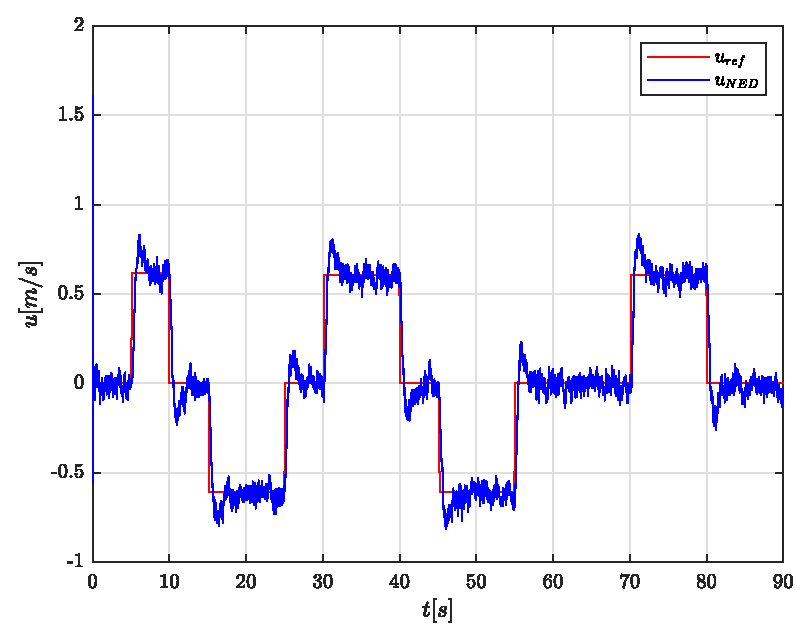
\includegraphics[width=1\textwidth]{Simulazioni/Figure/PID/SNAKE_MIL/PositionControlXVel}
		\caption{Controllo velocità lungo x}
		\label{fig:SNAKEerrvelxPID_MIL}
	\end{subfigure}
	\hfill
	\begin{subfigure}{0.45\textwidth}
		\centering
		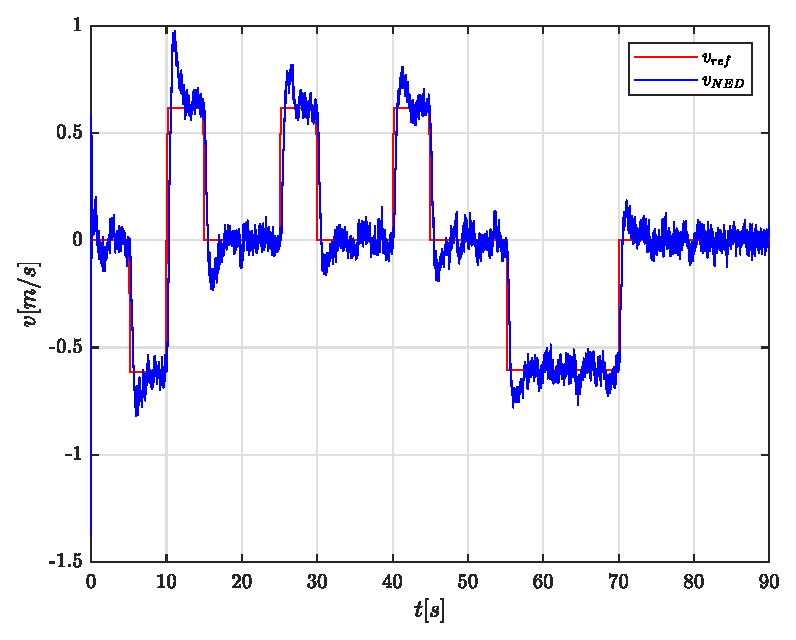
\includegraphics[width=1\textwidth]{Simulazioni/Figure/PID/SNAKE_MIL/PositionControlYVel}
		\caption{Controllo velocità lungo y}
		\label{fig:SNAKEerrvelyPID_MIL}
	\end{subfigure}
	\caption{Risposta nella simulazione MIL in velocità con controllore PID al comando SNAKE}
\end{figure}

Nel comando in termine di velocità mediamente il segnale viene inseguito correttamente, con la presenza però di un rumore nella posizione effettiva, Figure (\ref{fig:SNAKEerrvelxPID_MIL}) e (\ref{fig:SNAKEerrvelyPID_MIL}). Questo effetto è dovuto alla presenza della derivata della velocità nel controllo di posizione, che amplifica l'errore di misurazione della velocità.

\begin{figure}
	\centering
	\begin{subfigure}{0.45\textwidth}
		\centering
		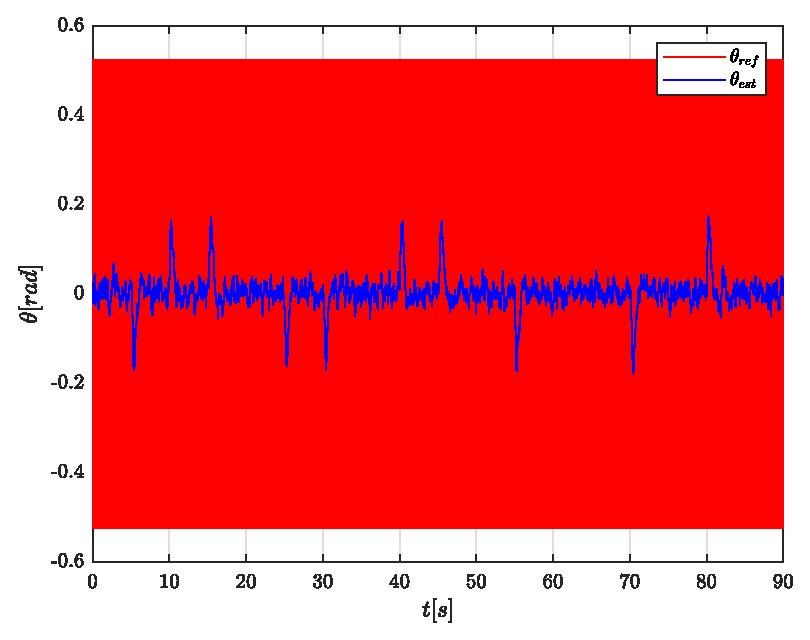
\includegraphics[width=1\textwidth]{Simulazioni/Figure/PID/SNAKE_MIL/AttitudeControlPitch}
		\caption{Controllo beccheggio}
		\label{fig:SNAKEbecPID_MIL}
	\end{subfigure}
	\hfill
	\begin{subfigure}{0.45\textwidth}
		\centering
		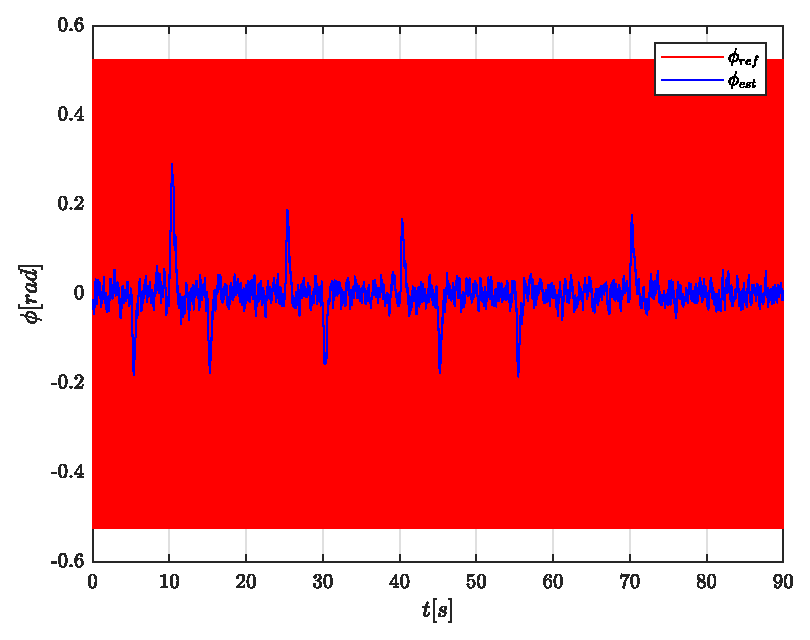
\includegraphics[width=1\textwidth]{Simulazioni/Figure/PID/SNAKE_MIL/AttitudeControlRoll}
		\caption{Controllo rollio}
		\label{fig:SNAKErolPID_MIL}
	\end{subfigure}
	\hfill
	\begin{subfigure}{0.45\textwidth}
		\centering
		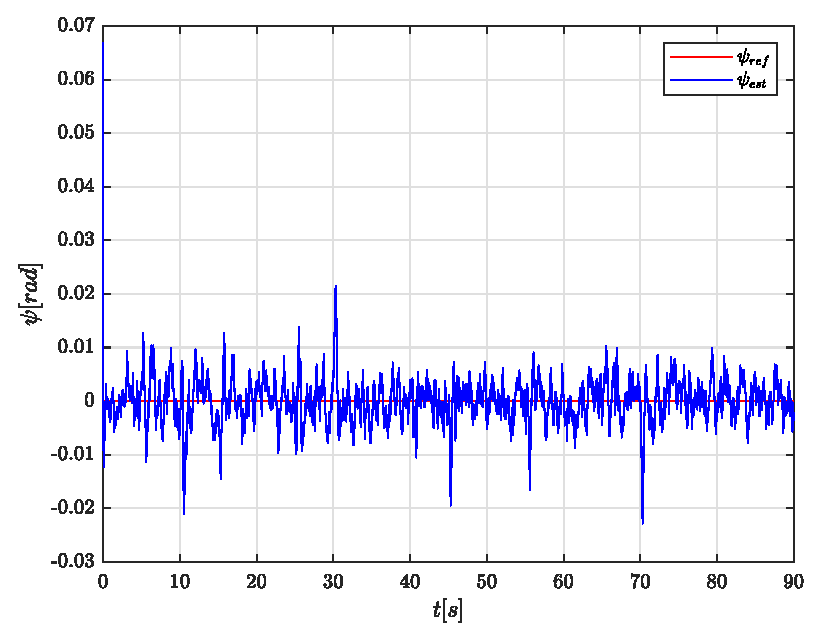
\includegraphics[width=1\textwidth]{Simulazioni/Figure/PID/SNAKE_MIL/AttitudeControlYaw}
		\caption{Controllo imbardata}
		\label{fig:SNAKEyawPID_MIL}
	\end{subfigure}
	\caption{Risposta dell' assetto nella simulazione MIL con controllore PID al comando SNAKE}
\end{figure}

Osservando infatti il segnale comandato dal sistema di controllo della posizione, Figure (\ref{fig:SNAKEbecPID_MIL}) e (\ref{fig:SNAKErolPID_MIL}), è chiaramente visibile l'amplificazione di questo errore, che porta in saturazione il comando in tutta la simulazione. Nelle stesse figure è visibile come il sistema risponda comunque in modo stabile mediando il valore di riferimento generato dal Position Control. Nella Figura (\ref{fig:SNAKEyawPID_MIL}), si osserva come il rumore introdotto dalla presenza della componente derivativa sulla velocità, attraverso l'azionamento dell'Attitude Control, venga portato per accoppiamento delle dinamiche anche sulla variazione dell'imbardata.

\begin{figure}
	\centering
	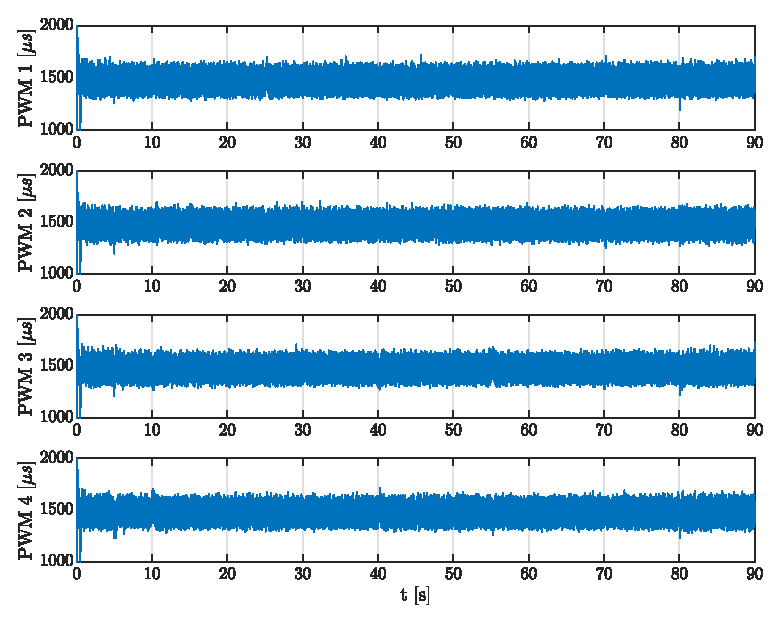
\includegraphics[width=0.5\textwidth]{Simulazioni/Figure/PID/SNAKE_MIL/PWM}
	\caption{Segnali PWM del controllore PID al segnale SNAKE}
	\label{fig:SNAKEPWMPID_MIL}
\end{figure}

Analizzando il segnale PWM generato, Figura (\ref{fig:SNAKEPWMPID_MIL}), si osserva il comando con una componente oscillatoria costante per tutta la simulazione, rimanendo pero nei limiti di saturazione.

\subsection{SMC}
Nella seguente simulazione si utilizza il controllore SMC ripercorrendo lo stesso percorso della sezione precedente.

\begin{figure}
	\centering
	\begin{subfigure}{0.45\textwidth}
		\centering
		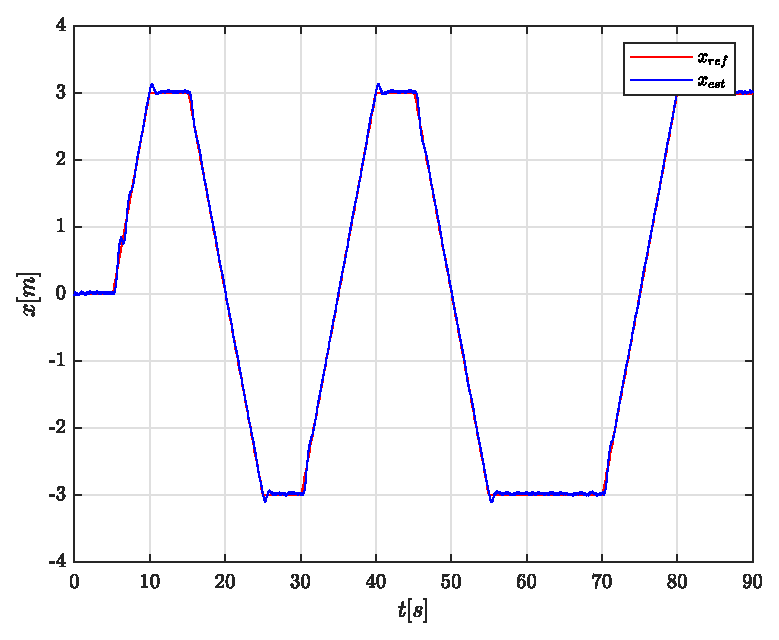
\includegraphics[width=1\textwidth]{Simulazioni/Figure/SMC/SNAKE_MIL/PositionControlXPos}
		\caption{Controllo posizione lungo x}
		\label{fig:SNAKEerrposxSMC_MIL}
	\end{subfigure}
	\hfill
	\begin{subfigure}{0.45\textwidth}
		\centering
		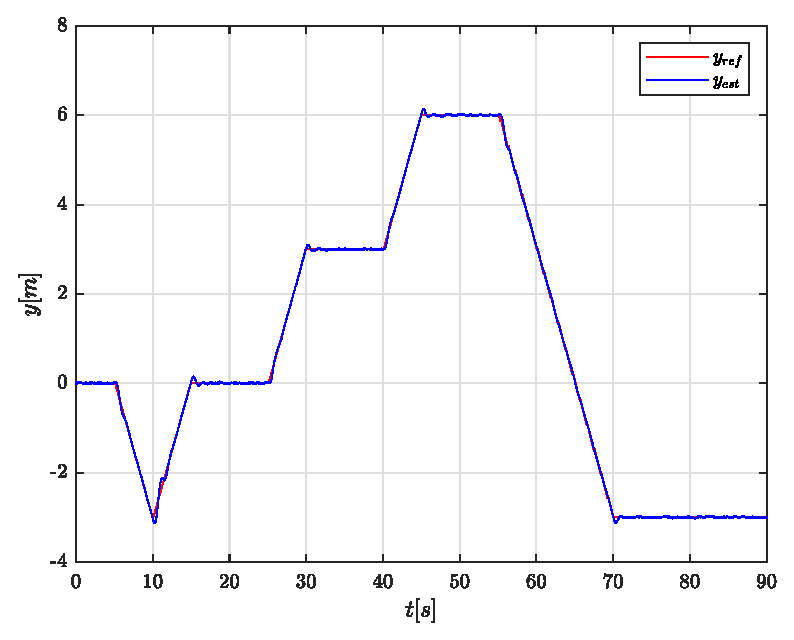
\includegraphics[width=1\textwidth]{Simulazioni/Figure/SMC/SNAKE_MIL/PositionControlYPos}
		\caption{Controllo posizione lungo y}
		\label{fig:SNAKEerrposySMC_MIL}
	\end{subfigure}
	\caption{Risposta in posizione nella simulazione MIL con controlloreSMC al comando SNAKE}
\end{figure}

Anche in questa simulazione è visibile l'efficacia del sistema di controllo nell'inseguimento della posizione di riferimento, Figure (\ref{fig:SNAKEerrposxSMC_MIL}) e (\ref{fig:SNAKEerrposySMC_MIL}). Analogamente alla simulazione precedente il segnale di velocità è mediamente seguito correttamente, con la presenza di un oscillazione di ampiezza contenuta docuta questa volta al tipo di comando discontinuo del controllore SMC, Figure (\ref{fig:SNAKEevelxSMC_MIL}) e (\ref{fig:SNAKEevelySMC_MIL}). In definitiva la traiettoria è seguita in modo efficace, Figura (\ref{fig:SNAKEetraSMC_MIL}).

\begin{figure}
	\centering
	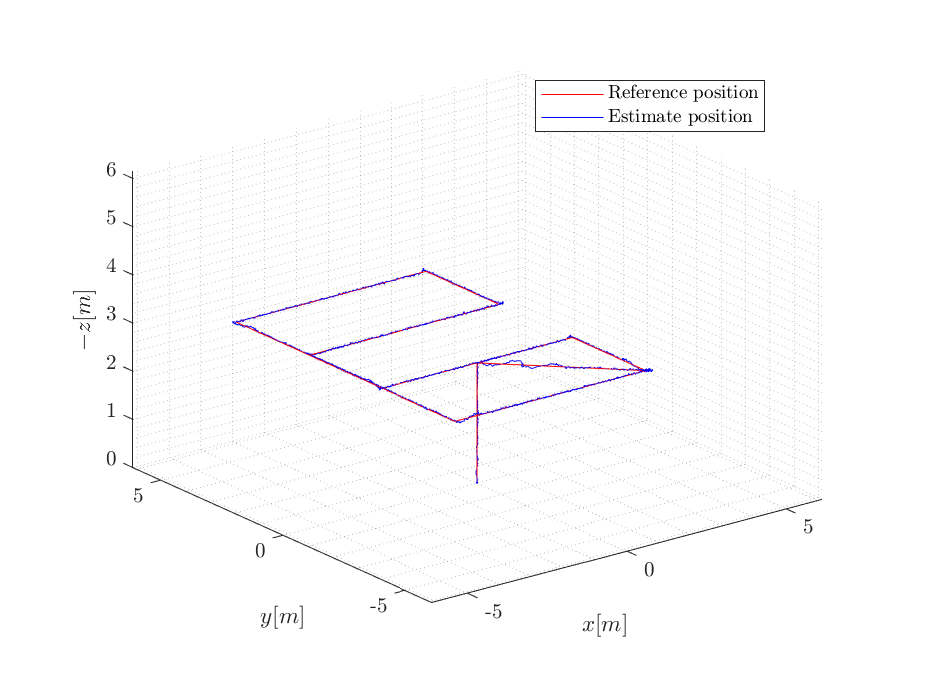
\includegraphics[width=0.65\textwidth]{Simulazioni/Figure/SMC/SNAKE_MIL/Trajectory}
	\caption{Traiettoria percorsa con controllore SMC nella simulazione MIL al segnale SNAKE}
	\label{fig:SNAKEetraSMC_MIL}
\end{figure}

\begin{figure}
	\centering
	\begin{subfigure}{0.45\textwidth}
		\centering
		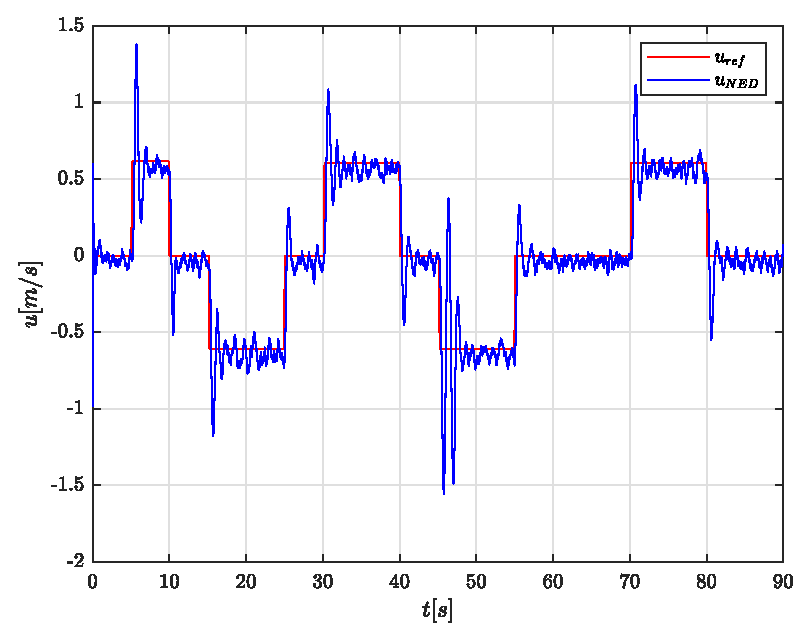
\includegraphics[width=1\textwidth]{Simulazioni/Figure/SMC/SNAKE_MIL/PositionControlXVel}
		\caption{Controllo velocità lungo x}
		\label{fig:SNAKEevelxSMC_MIL}
	\end{subfigure}
	\hfill
	\begin{subfigure}{0.45\textwidth}
		\centering
		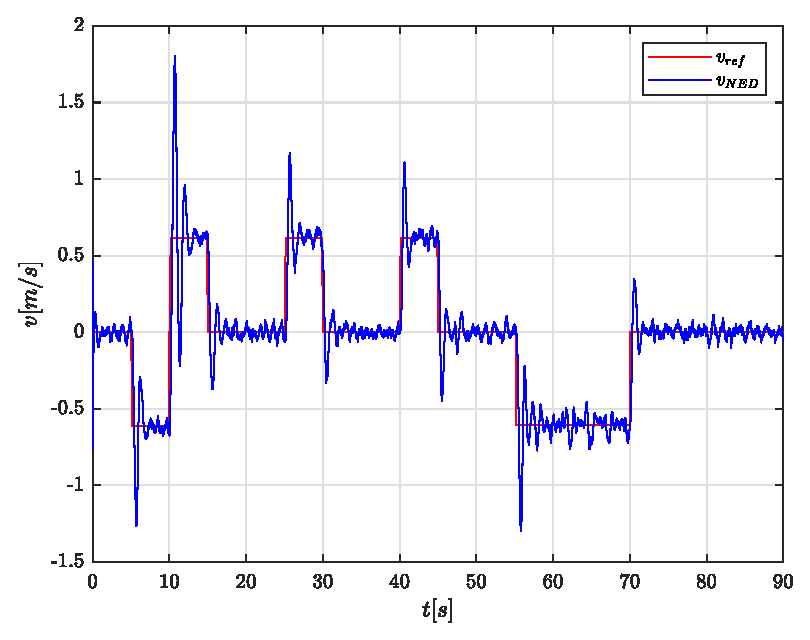
\includegraphics[width=1\textwidth]{Simulazioni/Figure/SMC/SNAKE_MIL/PositionControlYVel}
		\caption{Controllo velocità lungo y}
		\label{fig:SNAKEevelySMC_MIL}
	\end{subfigure}
	\caption{Risposta in velocità nella simulazione MIL con controlloreSMC al comando SNAKE}
\end{figure}

\begin{figure}
	\centering
	\begin{subfigure}{0.45\textwidth}
		\centering
		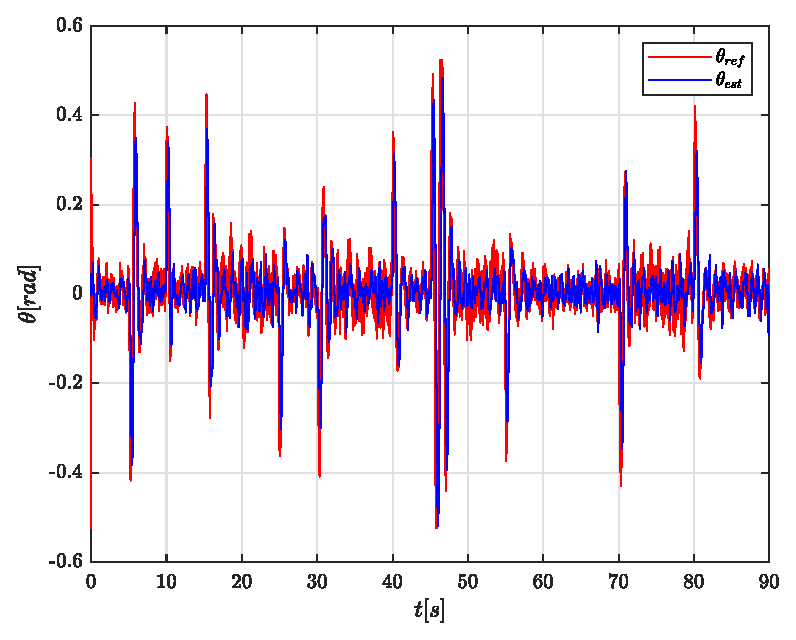
\includegraphics[width=1\textwidth]{Simulazioni/Figure/SMC/SNAKE_MIL/AttitudeControlPitch}
		\caption{Controllo beccheggio}
		\label{fig:SNAKEbecSMC_MIL}
	\end{subfigure}
	\hfill
	\begin{subfigure}{0.45\textwidth}
		\centering
		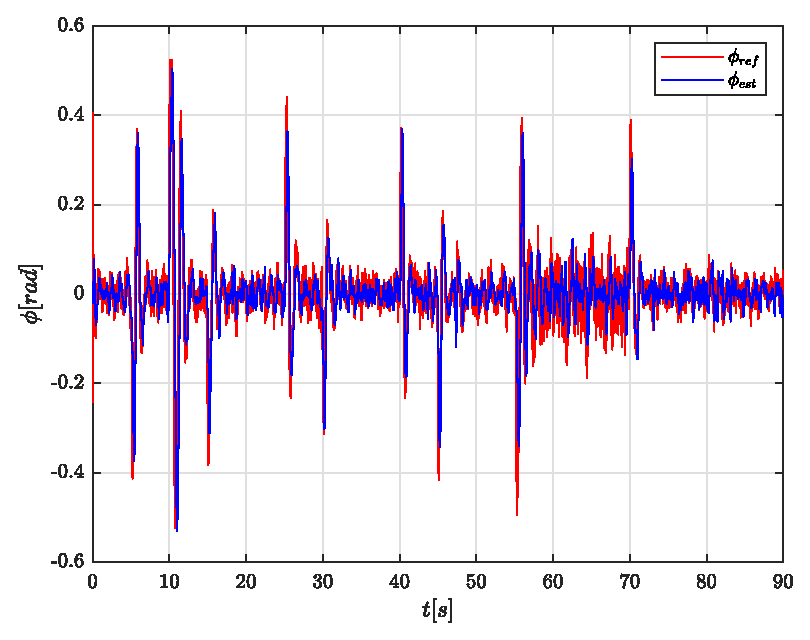
\includegraphics[width=1\textwidth]{Simulazioni/Figure/SMC/SNAKE_MIL/AttitudeControlRoll}
		\caption{Controllo rollio}
		\label{fig:SNAKErolSMC_MIL}
	\end{subfigure}
	\hfill
	\begin{subfigure}{0.45\textwidth}
		\centering
		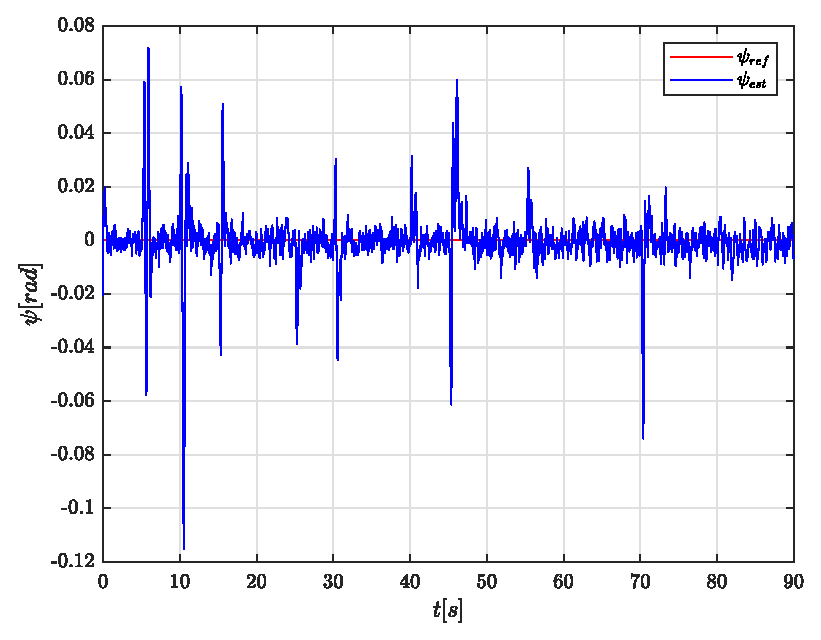
\includegraphics[width=1\textwidth]{Simulazioni/Figure/SMC/SNAKE_MIL/AttitudeControlYaw}
		\caption{Controllo imbardata}
		\label{fig:SNAKEyawSMC_MIL}
	\end{subfigure}
	\caption{Risposta dell' assetto nella simulazione MIL con controllore SMC al comando SNAKE}
\end{figure}

In questo caso il sistema di Position Control presenta solo piccole porzioni di saturazione, con un segnale di riferimento contenente una componente oscillatoria dovuta al controllo SMC ed una risposta molto precisa, Figure (\ref{fig:SNAKEbecSMC_MIL}) e (\ref{fig:SNAKEbecSMC_MIL}). \'E possibile vedere nella Figura (\ref{fig:SNAKEyawSMC_MIL}), l'effetto di accoppiamento delle rotazioni nella risposta del sistema relativa all'angolo di imbardata.

\begin{figure}
	\centering
	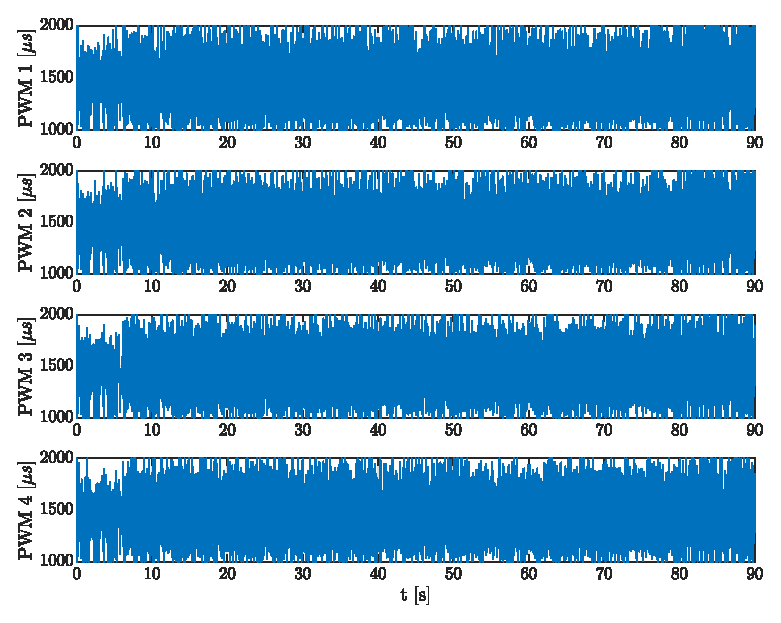
\includegraphics[width=0.5\textwidth]{Simulazioni/Figure/SMC/SNAKE_MIL/PWM}
	\caption{Segnali PWM del controllore SMC al segnale SNAKE}
	\label{fig:SNAKEPWMSMC_MIL}
\end{figure}

Terminando, il segnale generato da questo controllo presenta una chiara discontinuità e presenza di saturazione nel riferimento generato per il comando PWM, Figura (\ref{fig:SNAKEPWMSMC_MIL}).

\subsection{Confronto}

I due sistemi di controllo riportati in queste simulazioni MIL, sono entrambi efficaci nel controllare il velivolo durante la missione assegnata. Il comando generato dal Position controller utilizzando il sistema di controllo con SMC risulta essere migliore, Figure (\ref{fig:SNAKEbecPID_MIL}), (\ref{fig:SNAKErolPID_MIL}), (\ref{fig:SNAKEbecSMC_MIL}) e ((\ref{fig:SNAKErolSMC_MIL})). Il segnale finale PWM però generato dal sistema SMC, come nel caso della simulazione SIL, risulta essere più impegnativo in termini di attuazione, rispetto il sistema di controllo PID, Figure (\ref{fig:SNAKEPWMPID_MIL}) e (\ref{fig:SNAKEPWMSMC_MIL}).

Vengono determinati i valori degli errori di posizione massimo e medio, come analogamente fatto per simulazioni SIl, attraverso le formulazioni (\ref{eq:err_max}) e (\ref{eq:err_med}), riportando i risultati numerici nella Tabella (\ref{tab:ConfrontoPIDSMCMIL}). I risultati sono invece rappresentati nella Figura (\ref{fig:erroriMIL}).

\begin{figure}
	\centering
	\begin{subfigure}{0.48\textwidth}
		\centering
		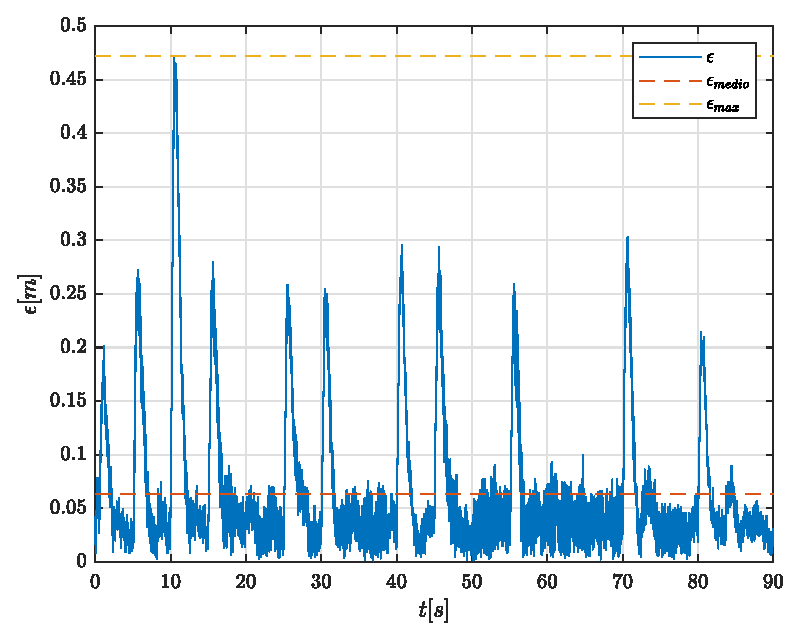
\includegraphics[width=1\textwidth]{Simulazioni/Figure/PID/SNAKE_MIL/ERR}
		\caption{Controllore PID}
	\end{subfigure}
	\hfill
	\begin{subfigure}{0.48\textwidth}
		\centering
		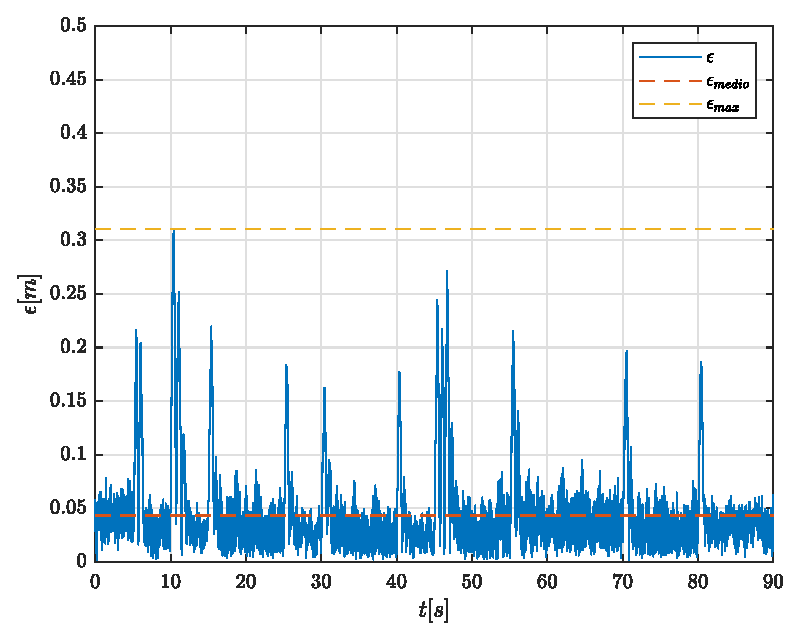
\includegraphics[width=1\textwidth]{Simulazioni/Figure/SMC/SNAKE_MIL/ERR}
		\caption{Controllore SMC}
	\end{subfigure}
	\caption{Errori di posizione tra PID e SMC nel tempo nelle simulazioni MIL}
	\label{fig:erroriMIL}
\end{figure}

\begin{table}
	\centering
	\caption{Errori di posizione al comando SNAKE attraverso simulazione SIL}
	\begin{tabular}{c c c}
		\hline
		Errore &  PID [m] & SMC [m] \\
		\hline
		$\epsilon_{max}$ & 0.47 & 0.31  \\
		$\epsilon_{medio}$ & 0.06 & 0.04  \\
		\hline
	\end{tabular}	
	\label{tab:ConfrontoPIDSMCMIL}
\end{table}

Confrontando le Figure (\ref{fig:errori}), (\ref{fig:erroriMIL}) e le relative Tabelle (\ref{tab:ConfrontoPIDSMCSIL}), (\ref{tab:ConfrontoPIDSMCMIL}), si constata l'effettiva similarità tra le simulazioni SIL e MIL. Le simulazioni MIL mostrano dei valori di errore leggermente minori rispetto a quelli ottenuti dalle simulazioni SIL. Questo è fondamentalmente dovuto al fatto che nel MIL non si è tenuto conto del campionamento dei segnali. Nell'esecuzione del software è necessario generare e condividere i messaggi attraverso i protocolli MAVLink e $\micro$ORB, in modo da poter eseguire concorrenzialmente i moduli presenti all'interno del firmware PX4 e scambiare i dati con i componenti simulati su Gazebo. Questi fattori comportano un campionamento dei segnali più grossolano per rispettare la rapidità di esecuzione, con l'effetto equivalente ad un filtraggio delle variazioni ad alta frequenza. Specialmente nel caso del controllore PID, questo effetto riduce l'effetto del rumore introdotto dalla misurazione delle velocità e delle velocità angolari utilizzate, con il relativo miglioramento in termine di prestazione. Nel controllore SMC questo effetto è poco rilevabile in termini di misura di errore a causa della sua intrinseca robustezza, ma pienamente apprezzabile nella presenza di forti discontinuità nel comando PWM generato, (\ref{fig:SNAKEPWMSMC_MIL}).